\documentclass{article}

\usepackage[english]{babel}
\usepackage{amsthm}
\usepackage{float}
\usepackage{amsmath} % for theorems
\usepackage{mathtools}
\usepackage{amssymb}
\usepackage{xfrac} % for nice fractions
\usepackage[utf8]{inputenc} % allow utf-8 input
\usepackage[T1]{fontenc}    % use 8-bit T1 fonts
\usepackage{hyperref}       % hyperlinks
\usepackage{url}            % simple URL typesetting
\usepackage{booktabs}       % professional-quality tables
\usepackage{amsfonts}       % blackboard math symbols
\usepackage{nicefrac}       % compact symbols for 1/2, etc.
\usepackage{microtype}      % microtypography
\usepackage{lipsum}
\usepackage{fancyhdr}       % header
\usepackage{graphicx}       % graphics
\usepackage{xcolor}         % colors
\usepackage{subcaption}
\usepackage{booktabs}

\usepackage{todonotes}
\newcommand{\aanote}[1]{\todo[color=blue!35]{\small AA: #1}}
\newcommand{\dd}{\mathrm d}

\newcommand{\theHalgorithm}{\arabic{algorithm}}

\usepackage[preprint]{neurips_2026}

\usepackage[capitalize,noabbrev]{cleveref}

%%%%%%%%%%%%%%%%%%%%%%%%%%%%%%%%
% THEOREMS
%%%%%%%%%%%%%%%%%%%%%%%%%%%%%%%%
\theoremstyle{plain}
\newtheorem{theorem}{Theorem}[section]
\newtheorem{proposition}[theorem]{Proposition}
\newtheorem{lemma}[theorem]{Lemma}
\newtheorem{corollary}[theorem]{Corollary}
\theoremstyle{definition}
\newtheorem{definition}[theorem]{Definition}
\newtheorem{assumption}[theorem]{Assumption}
\theoremstyle{remark}
\newtheorem{remark}[theorem]{Remark}

\newcommand{\prefactor}[2]{A_{#1,#2}}
\DeclareMathOperator*{\argmin}{arg\,min}

\title{Global Optimization via Softmin energy Minimization}


\author{
Samuele Saviozzi \\
Department of Mathematics\\
University of Pisa\\
Pisa, Italy \\
\texttt{samuele.saviozzi@phd.unipi.it} \\
\And
Andrea Agazzi \\
Institute of Mathematical Statistics \\and Actuarial Science\\ 
University of Bern\\
Bern, Switzerland\\
\texttt{andrea.agazzi@unibe.ch} \\
\AND
Vittorio Carlei \\
Department of Business Economics\\ 
University Gabriele D'annunzio\\
Chieti, Italy
\texttt{carlei@unich.it} \\
\And
Marco Romito \\
Department of Mathematics\\
University of Pisa\\
Pisa, Italy \\
\texttt{marco.romito@unipi.it} \\
}

% The \author macro works with any number of authors. There are two commands
% used to separate the names and addresses of multiple authors: \And and \AND.
%
% Using \And between authors leaves it to \LaTeX{} to determine where to break
% the lines. Using \AND forces a linebreak at that point. So, if \LaTeX{}
% puts 3 of 4 authors names on the first line, and the last on the second
% line, try using \AND instead of \And before the third author name.

\newcommand{\fix}{\marginpar{FIX}}
\newcommand{\new}{\marginpar{NEW}}

%\nipsfinalcopy % Uncomment for camera-ready version

\begin{document}

%\DeclareMathSizes{10}{8}{6}{4}

% \icmltitlerunning{Global Optimization via Softmin energy Minimization}

% \begin{document}

% \twocolumn[
%     \icmltitle{Global Optimization via Softmin energy Minimization}

%     \begin{icmlauthorlist}
%         \icmlauthor{Samuele Saviozzi}{pisa}
%         \icmlauthor{Andrea Agazzi}{berna}
%         \icmlauthor{Marco Romito}{pisa}
%         \icmlauthor{Vittorio Carlei}{chieti}
%     \end{icmlauthorlist}

%     \icmlaffiliation{pisa}{Department of Mathematics, University of Pisa, Pisa, Italy}
%     \icmlaffiliation{berna}{Institute of Mathematical Statistics and Actuarial Science, University of Bern, Bern, Switzerland}
%     \icmlaffiliation{chieti}{Department of Business Economics, University Gabriele D'annunzio, Chieti, Italy}

%     \icmlcorrespondingauthor{Samuele Saviozzi}{samuele.saviozzi@phd.unipi.it}
%     \icmlcorrespondingauthor{Andrea Agazzi}{andrea.agazzi@unibe.ch}

%     \icmlkeywords{Particle Swarm, Non-convex Optimization, Stochastic Particles Methods, Boltzmann Energy}

%     \vskip 0.3in
%     ]

% \printAffiliationsAndNotice{}

\maketitle

\begin{center}
\fbox{\parbox{0.94\linewidth}{\textbf{Working major-revision draft.} The theoretical statements have been narrowed to remove the contradictions identified in review. The numerical section contains explicit author notes and must be completed with new experiments before resubmission.}}
\end{center}

\begin{abstract}
We study a fixed-population Langevin system on particle space whose potential is the Gibbs-weighted objective average
\(J_\beta(\mathbf{x})=\sum_i w_i(\mathbf{x})f(x_i)\).  Its component drift is a scalar multiple of \(-\nabla f(x_i)\), and the scalar changes sign according to the particle's objective value relative to the ensemble.  We first characterize the equilibria of the joint potential without imposing convexity: consensus at any strict local minimum of \(f\) is locally stable, whereas every equilibrium containing a noncritical zero-rate particle is unstable.  We then prove that the best objective value in the deterministic ensemble decreases at least as fast as ordinary gradient flow under a Polyak--\L{}ojasiewicz condition; this statement is ensemble-level and does not assume that the other particles are stationary.  Finally, in one dimension and for fixed \(\beta\), we derive an explicit \(O(\beta^{-1})\) upper bound on the Freidlin--Wentzell exponent for the first exit of the joint diffusion from a local basin.  This is an upper-bound result, not an Eyring--Kramers prefactor formula and not a proof of global convergence.  Numerical experiments are designed to test the sign-changing drift mechanism, sensitivity to particle count and temperature, and performance under matched objective/gradient-evaluation budgets.
\end{abstract}

% \section{Introduction}
% Non-convex optimization problems are notoriously difficult, as the presence of multiple local minima can trap gradient-based algorithms. Existing approaches such as gradient descent perform well for convex functions with a single minimum but will likely converge to suboptimal local minima in more complex landscapes. This challenge is especially prominent in machine learning, where training deep neural networks on non-convex losses often leads to inconsistent performance across random initializations. Similarly, in reinforcement learning, escaping sharp local minima remains a key bottleneck for achieving state-of-the-art results. 

% A classical strategy to address this issue is to add a noise term to the dynamics, allowing the system to escape local minima and leading to stochastic gradient–based methods, for example Langevin dynamics \cite{CoffeyKalmykovWaldron2004}. Stochastic gradient-based methods for optimization, while effective, typically exhibit poor transition times between local minima. The escape rate of a particle subject to Gaussian noise from a local minimum depends exponentially on the height of the potential barrier surrounding that minimum \cite{berglund2011kramers}. Methods that improve convergence rates over gradient-based algorithms often rely on additional assumptions about the objective function $f$. For example, if $f$ admits a decomposition as a linear combination of simpler functions $\psi_i$, i.e., $f(x) = \sum_i \psi_i(x)$, then the Method of Moments \cite{meziat2003method} can be employed to converge to the global minimum. This type of decomposition is particularly useful in areas such as signal processing and machine learning, where complex functions are represented as sums of basis functions, such as Fourier series or wavelets \cite{shao1993signal}. In more general settings where such structure is not available, Simulated Annealing and its variants \cite{bolte2024swarm,xu2018global} are widely used, leveraging a decaying temperature schedule to shift the dynamics from noisy exploration to refined local search.

% A natural extension of stochastic gradient-based approaches is the use of multiple particles to explore the search space in parallel. For instance, when particles evolve independently under Langevin dynamics, the expected transition times between local minima decrease compared to single-particle dynamics purely due to statistical averaging over multiple independent trajectories. Moreover, allowing particles to cooperate rather than evolve independently can further improve exploration and convergence. The idea of particle cooperation is often central in Metaheuristic methods \cite{bandaru2016metaheuristic,yang2020nature}. Such methods provide a broad framework for global optimization and have demonstrated strong empirical performance, although establishing rigorous theoretical convergence guarantees is often challenging. Many such methods employ a particle-swarm-like paradigm \cite{hussain2019metaheuristic,rajwar2023exhaustive}, in which multiple interacting particles explore the search space in parallel to locate global minimizers.

% The global optimization method proposed in this paper builds on these ideas by combining stochastic gradient techniques with cooperative multi-particle dynamics. We employ the well-known Softmin energy functional $J_\beta$, which smoothly interpolates between the average and the hard minimum of the function values across particle positions. This functional acts as the source of interaction among particles, whose evolution is governed by its gradient, driving the system toward more effective exploration and optimization.

% The Softmin function provides a natural way to interpolate between uniform weighting and hard minima via temperature $\beta>0$. A common use of the Softmin function is to define the Gibbs distribution, where the probability of sampling $x_i$ is given by: 
% \[
%     \mathbb{P}[i] = \tfrac{\exp{(-\beta{x_i})}}{\sum_{j=1}^n \exp{(-\beta x_j})},
% \] 
% with $\beta\to\infty$ concentrating on $\min_{i} x_i$ and $\beta\to0$ uniform \cite{bertsekas1997nonlinear}. This underlies stochastic optimization \cite{ackley1985boltzmann, srivastava2012multimodal, gelfand1990sampling,gelfand2000gibbs} and exploration in Reinforcement Learning \cite{pan2019reinforcement, haarnoja2017reinforcement}.

% Our proposed method is a stochastic gradient-based particle swarm approach that leverages a Softmin-type energy functional to effectively incorporate gradient information from the particles. Consider a differentiable function $f:\mathbb{R}^d\to\mathbb{R}$. The objective is to approximately solve the global minimization problem $\min_{x\in\mathbb{R}^d}f(x)$. Given a population of $n$ particles $\mathbf{x}=(x_1,\dots,x_n)$ with $x_i\in\mathbb{R}^d$ for all $i\in[n]$, the Softmin energy is defined as: 
% \begin{equation}
%     J_\beta(\mathbf{x})=\sum_{i=1}^n\frac{\exp(-\beta f(x_i))}{\sum_{j=1}^n\exp(-\beta f(x_j))}f(x_i),
%     \label{eq:Softmin-energy}
% \end{equation}
% which provides a smooth approximation of the empirical minimum among the $f(x_i)$. The parameter $\beta>0$ controls the approximation's sharpness: larger values yield a closer approximation to the hard minimum $\min_i f(x_i)$, while $\beta\to0$ recovers the average $\frac 1 n \sum_{i=1}^n f(x_i)$. 

% To minimize $J_\beta$ we consider the stochastic gradient flow in the particle space $\mathbb{R}^{nd}$: 
% \begin{equation}\label{e:sde}
%    d\mathbf{x}_t = -n\nabla J_{\beta_t}(\mathbf{x}_t)dt+\sqrt{2\sigma}dB_t, 
% \end{equation} 
% where $(B_t)_{t\geq 0}$ represents a standard $nd$-dimensional Brownian motion and $\sigma>0$ introduces stochasticity to promote exploration and escape from local minima.

% \subsection{Contribution}
% The dynamics in \eqref{e:sde} are an overdamped Langevin diffusion on the extended space \(\mathbb{R}^{nd}\) with joint potential \(U_\beta=nJ_\beta\).  Our contribution is therefore not the use of Langevin dynamics per se, but the analysis of this particular nonseparable potential and of the sign-changing component drift that it induces.

% \paragraph{Equilibrium geometry and role assignment.}
% Writing
% \[
%  a_k(\mathbf{x}) := n w_k(\mathbf{x})\bigl[1-\beta(f(x_k)-J_\beta(\mathbf{x}))\bigr],
% \]
% the deterministic component equation is \(\dot x_k=-a_k(\mathbf{x})\nabla f(x_k)\).  We characterize all equilibria and show that consensus at a nondegenerate critical point has exactly the same local stability type as that critical point of \(f\).  In contrast, an equilibrium containing a noncritical particle with \(a_k=0\) has a negative Hessian direction and is unstable.  No global or ``local on every compact set'' convexity assumption is used.

% \paragraph{Best-particle descent under joint evolution.}
% The sign of \(a_k\) is not invariant for a fixed particle because all coordinates enter \(J_\beta\).  The correct invariant statement is ensemble-level: every particle attaining the current minimum objective value satisfies \(a_k\ge 1\).  Consequently, under a Polyak--\L{}ojasiewicz inequality on the relevant sublevel set, the best objective value decays at least at the ordinary gradient-flow rate.

% \paragraph{A computable basin-exit upper bound.}
% For fixed \(\beta\), freezing \(n-1\) particles at a local minimizer reduces the joint potential along a one-particle path to
% \[
%  u_{n,\beta}(r)=\frac{n r e^{-\beta r}}{n-1+e^{-\beta r}}.
% \]
% Its global maximum is \(B_{n,\beta}=n(y_n-1)/\beta< n/[e(n-1)\beta]\), where \(y_n\) is the unique solution of \(y=1+e^{-y}/(n-1)\).  In the one-dimensional adjacent-well setting, this gives a Freidlin--Wentzell upper bound on the first basin-exit exponent.  We deliberately do not claim an exact Eyring--Kramers formula, one-particle channel dominance, or global convergence.

% \subsection{Related work}

% \paragraph{Langevin and stochastic-gradient Langevin methods.}
% Equation \eqref{e:sde} belongs to the broad family of Langevin diffusions.  Stochastic-gradient Langevin dynamics was introduced for scalable Bayesian learning by Welling and Teh \cite{welling2011bayesian}, and nonasymptotic guarantees for nonconvex learning were developed by Raginsky, Rakhlin, and Telgarsky \cite{raginsky2017nonconvex}.  These methods generally use a single objective on the original parameter space, whereas our drift is the gradient of a nonseparable potential on the product space.  The distinction is the potential geometry, not the stochastic-differential-equation template.

% \paragraph{Interacting-particle Langevin algorithms.}
% Interacting-particle Langevin algorithms (IPLA) also formulate Langevin diffusions on extended particle spaces and provide rigorous nonasymptotic analyses, notably for maximum marginal likelihood in latent-variable models \cite{akyildiz2025interacting}; proximal variants address nonsmooth latent-variable models \cite{encinar2025proximal}.  These works are mathematically closer to the present paper than generic swarm heuristics and must be treated as primary related work.  Their interactions arise from latent-variable likelihood structure and target statistical estimation, while the present potential is the Gibbs-weighted objective average \(J_\beta\) and is introduced to create sign-changing optimization roles.  This is a difference in interaction design and target problem, not a claim that the methods lie in unrelated algorithmic classes.

% \paragraph{Consensus, particle-swarm, and swarm-gradient optimization.}
% Consensus-based optimization (CBO) \cite{CarrilloChoiTotzeckTse2018,pinnau2017consensus,carrillo2021consensus,fornasier2024consensus}, particle swarm optimization (PSO) \cite{kennedy1995particle,noel2012new}, and swarm-gradient dynamics \cite{bolte2024swarm,riedl2023gradient} combine population information with local or stochastic motion.  CBO coordinates particles through a Gibbs-weighted spatial consensus and is typically gradient-free; PSO uses personal and global best positions; swarm-gradient methods derive gradient-like population dynamics and global-convergence mechanisms.  Our method instead takes gradient descent of the scalar joint functional \(J_\beta\).  Its distinctive algebraic feature is
% \(\nabla_{x_k}J_\beta=(a_k/n)\nabla f(x_k)\), so the interaction changes the sign and magnitude of the local gradient without introducing a consensus position.

% \paragraph{Scope of the novelty claim.}
% The paper claims novelty only for using the Gibbs-weighted objective average \(J_\beta\) itself as the joint potential and for the resulting equilibrium and barrier calculations.  It does not claim novelty for extended-space Langevin dynamics, Gibbs weights, stochastic-gradient noise, or population-based global search.

% \subsection{Structure of the paper}
% Section \ref{sec:gradient-flow-dynamics} derives the component dynamics and characterizes equilibria without convexity.  Section \ref{sec:one-dimensional-passage} gives two conservative guarantees: an upper bound on the fixed-temperature basin-exit exponent and an ensemble-level descent estimate for the best particle.  Section \ref{sec:numerical-experiments} specifies a cost-matched evaluation protocol and mechanism-focused ablations.  Technical proofs are collected in Appendix \ref{apx:technical-proofs}.

\section{Deterministic Softmin dynamics}
\label{sec:gradient-flow-dynamics}

For fixed \(\beta>0\), define the joint potential \(U_\beta(\mathbf{x})=nJ_\beta(\mathbf{x})\).  The deterministic dynamics are
\begin{equation}
    \dot{\mathbf{x}}_t=-\nabla U_\beta(\mathbf{x}_t)=-n\nabla J_\beta(\mathbf{x}_t).
    \label{eq:gradient-flow}
\end{equation}
Let
\[
 w_k(\mathbf{x})=\frac{e^{-\beta f(x_k)}}{\sum_{j=1}^n e^{-\beta f(x_j)}},
 \qquad
 a_k(\mathbf{x})=n w_k(\mathbf{x})\bigl[1-\beta(f(x_k)-J_\beta(\mathbf{x}))\bigr].
\]
A direct calculation gives
\begin{equation}
 \nabla_{x_k}J_\beta(\mathbf{x})=\frac{a_k(\mathbf{x})}{n}\nabla f(x_k),
 \qquad
 \dot x_k=-a_k(\mathbf{x})\nabla f(x_k).
 \label{eq:softmin-gradient}
\end{equation}
Thus \(a_k>0\) produces gradient descent and \(a_k<0\) produces gradient ascent.  This sign classification is instantaneous.  It is not, in general, invariant for a fixed particle because \(a_k\) depends on every particle coordinate.

\subsection{Equilibria and local stability}
\label{sec:stationary-points}

\begin{theorem}[Stability]
\label{thm:stable-stationary-points}
Let \(f\in C^2(\mathbb R^d)\), let \(\beta>0\), and consider the
gradient system
\[
    \dot{\mathbf x} = -n\nabla J_\beta(\mathbf x), \qquad \mathbf x=(x_1,\ldots,x_n)\in(\mathbb R^d)^n.
\]

Let
\[
    \bar{\mathbf x} = (\bar x_1,\ldots,\bar x_n)
\]
be a  stable equilibrium. Then, for every \(k\in\{1,\ldots,n\}\),

\begin{enumerate}
    \item \(\nabla f(\bar x_k)=0\);
    \item \(a_k(\bar{\mathbf x})\neq0\);
    \item the type of the critical point \(\bar x_k\) is compatible with the sign of \(a_k(\bar{\mathbf x})\):
    \[
        \begin{cases}
        \bar x_k \text{ is a local minimum of }f, & a_k(\bar{\mathbf x})>0,\\[1mm]
        \bar x_k \text{ is a local maximum of }f, & a_k(\bar{\mathbf x})<0.
        \end{cases}
    \]
\end{enumerate}
Moreover, every stable equilibrium contains at least one particle located at a local minimum of \(f\).
\end{theorem}
\begin{proof}
    See the appendix.
\end{proof}

\section{One-dimensional basin exit and post-saddle passage}
\label{sec:one-dimensional-passage}

% For the theoretical results in this section, \(\beta\) is fixed.  The time-inhomogeneous case \(\beta=\beta_t\) requires a separate analysis and is used only as an empirical heuristic in Section \ref{sec:numerical-experiments}.  The stochastic dynamics are
% \begin{equation}
%  d\mathbf{X}_t=-\nabla U_\beta(\mathbf{X}_t)\,dt+\sqrt{2\sigma}\,d\mathbf{B}_t,
%  \label{eq:gradient-flow-noisy}
% \end{equation}
% with \(U_\beta=nJ_\beta\).

\subsection{Freidlin--Wentzell framework}

Throughout this subsection, \(n\ge2\), the inverse temperature \(\beta>0\) is fixed, and the physical dimension is \(d=1\). The joint particle dynamics are
\begin{equation}
    d\mathbf X_t^\sigma
    =
    -\nabla U_\beta(\mathbf X_t^\sigma)\,dt
    +
    \sqrt{2\sigma}\,d\mathbf B_t,
    \qquad
    U_\beta(\mathbf x):=nJ_\beta(\mathbf x),
    \label{eq:joint-softmin-diffusion}
\end{equation}
with \(\mathbf X_t^\sigma\in\mathbb R^n\).

We consider three consecutive nondegenerate critical points
\[
    z_-<s<z_+,
\]
where \(z_-\) and \(z_+\) are local minima of \(f\), while \(s\) is the local maximum separating them. We assume
\begin{equation}
    f'(x)>0
    \quad\text{for }x\in(z_-,s),
    \qquad
    f'(x)<0
    \quad\text{for }x\in(s,z_+).
    \label{eq:adjacent-well-monotonicity}
\end{equation}
Set
\begin{equation}
    r(x):=f(x)-f(z_-),
    \qquad
    h:=r(s)>0,
    \qquad
    \rho_+:=r(z_+).
    \label{eq:relative-energy-coordinate}
\end{equation}

For an absolutely continuous path
\(\boldsymbol\phi:[0,T]\to\mathbb R^n\), the Freidlin--Wentzell action associated with \eqref{eq:joint-softmin-diffusion} is
\begin{equation}
    I_{0T}^\beta(\boldsymbol\phi)
    :=
    \frac14\int_0^T
    \left\|
        \dot{\boldsymbol\phi}(t)
        +
        \nabla U_\beta(\boldsymbol\phi(t))
    \right\|^2dt.
    \label{eq:fw-action}
\end{equation}
For a closed set \(A\subset\mathbb R^n\), define the quasipotential
\begin{equation}
    V_\beta(\mathbf x,A)
    :=
    \inf_{T>0}
    \inf_{\substack{
        \boldsymbol\phi(0)=\mathbf x\\
        \boldsymbol\phi(T)\in A
    }}
    I_{0T}^\beta(\boldsymbol\phi).
    \label{eq:fw-quasipotential}
\end{equation}
Under the standard hypotheses of Freidlin--Wentzell exit theory~\cite{freidlin2012random}, the expected exit time from a metastable domain \(D\) has exponential scale
\[
    \lim_{\sigma\downarrow0}
    \sigma\log\mathbb E_{\mathbf x}\tau_D^\sigma
    =
    V_\beta(\mathbf x,\partial D).
\]

The gradient structure is particularly useful. For every absolutely continuous path,
\begin{equation}
\begin{aligned}
    I_{0T}^\beta(\boldsymbol\phi)
    &=
    U_\beta(\boldsymbol\phi(T))
    -
    U_\beta(\boldsymbol\phi(0))
    \\
    &\quad+
    \frac14\int_0^T
    \left\|
        \dot{\boldsymbol\phi}(t)
        -
        \nabla U_\beta(\boldsymbol\phi(t))
    \right\|^2dt.
\end{aligned}
\label{eq:gradient-action-decomposition}
\end{equation}
Thus an uphill segment following the reversed gradient flow costs the corresponding increase in potential, whereas a downhill deterministic segment has zero action.

To construct an admissible escape path, freeze \(n-1\) particles at \(z_-\) and let one particle move:
\begin{equation}
    \Gamma(x):=(x,z_-,\ldots,z_-).
    \label{eq:frozen-background-channel}
\end{equation}
Along this channel, define
\begin{equation}
    u_{n,\beta}(r)
    :=
    \frac{nr e^{-\beta r}}{n-1+e^{-\beta r}},
    \qquad r\in\mathbb R.
    \label{eq:reduced-softmin-potential}
\end{equation}
The restriction of \(u_{n,\beta}\) to \([0,\infty)\) has a unique maximizer, denoted by
\(r_{n,\beta}^{\mathrm c}>0\). We write
\begin{equation}
    B_{n,\beta}
    :=
    u_{n,\beta}(r_{n,\beta}^{\mathrm c}),
    \qquad
    \widehat B_{n,\beta}(h)
    :=
    \max_{0\le r\le h}u_{n,\beta}(r).
    \label{eq:softmin-channel-barriers}
\end{equation}

\subsection{Theorem statement}

\begin{theorem}[One-dimensional basin exit and post-saddle passage]
\label{thm:transition-time}
Under the preceding assumptions, the following statements hold.

\begin{enumerate}
    \item Along the frozen-background channel,
    \begin{equation}
        U_\beta(\Gamma(x))-U_\beta(\Gamma(z_-))
        =
        u_{n,\beta}(r(x)).
        \label{eq:restricted-potential-identity}
    \end{equation}
    Moreover, \(u_{n,\beta}\) is strictly increasing on
    \([0,r_{n,\beta}^{\mathrm c}]\), strictly decreasing on
    \([r_{n,\beta}^{\mathrm c},\infty)\), and
    \begin{equation}
        B_{n,\beta}
        <
        \frac{n}{e(n-1)\beta}.
        \label{eq:reduced-barrier-cap}
    \end{equation}

    \item Let \(\bar{\mathbf z}_-:=\Gamma(z_-)\), and let \(x_-\in(z_-,s]\) be the unique point satisfying
    \[
        r(x_-)=\min\{h,r_{n,\beta}^{\mathrm c}\}.
    \]
    The minimum Freidlin--Wentzell action among paths constrained to \(\Gamma\) and joining \(\bar{\mathbf z}_-\) to \(\Gamma(s)\) is
    \begin{equation}
        V_{\beta,\mathrm{in}}^\Gamma
        =
        \widehat B_{n,\beta}(h)
        =
        \begin{cases}
            u_{n,\beta}(h),
            & h\le r_{n,\beta}^{\mathrm c},
            \\
            B_{n,\beta},
            & h>r_{n,\beta}^{\mathrm c}.
        \end{cases}
        \label{eq:initial-channel-action}
    \end{equation}
    Consequently,
    \begin{equation}
        V_\beta\bigl(\bar{\mathbf z}_-,\Gamma(x_-)\bigr)
        \le
        \widehat B_{n,\beta}(h),
        \qquad
        V_\beta\bigl(\bar{\mathbf z}_-,\Gamma(s)\bigr)
        \le
        \widehat B_{n,\beta}(h)
        <
        h.
        \label{eq:full-initial-quasipotential-bound}
    \end{equation}

    \item Assume in addition that
    \begin{equation}
        h>r_{n,\beta}^{\mathrm c},
        \qquad
        \rho_+<r_{n,\beta}^{\mathrm c}.
        \label{eq:high-barrier-regime}
    \end{equation}
    Then \(\mathbf s:=\Gamma(s)\) is a strict local minimum of the full joint potential \(U_\beta\). Let \(\xi_+\in(s,z_+)\) be the unique point satisfying
    \[
        r(\xi_+)=r_{n,\beta}^{\mathrm c}.
    \]
    The minimum action among channel paths joining \(\mathbf s\) to \(\Gamma(\xi_+)\) is
    \begin{equation}
        V_{\beta,\mathrm{post}}^\Gamma
        =
        B_{n,\beta}-u_{n,\beta}(h),
        \label{eq:post-saddle-channel-action}
    \end{equation}
    and therefore
    \begin{equation}
        V_\beta\bigl(\mathbf s,\Gamma(\xi_+)\bigr)
        \le
        B_{n,\beta}-u_{n,\beta}(h)
        <
        B_{n,\beta}.
        \label{eq:post-saddle-quasipotential-bound}
    \end{equation}
    Once the active particle crosses \(\xi_+\), the deterministic channel dynamics drive it toward \(z_+\).
\end{enumerate}
\end{theorem}

If \(D_-\subset\mathbb R^n\) is a metastable domain for the attractor \(\bar{\mathbf z}_-\), with \(\Gamma(x_-)\in\partial D_-\), and the standard Freidlin--Wentzell exit theorem applies, then
\begin{equation}
    \lim_{\sigma\downarrow0}
    \sigma\log
    \mathbb E_{\bar{\mathbf z}_-}\tau_{D_-}^\sigma
    =
    V_\beta(\bar{\mathbf z}_-,\partial D_-)
    \le
    \widehat B_{n,\beta}(h).
    \label{eq:initial-exit-time-bound}
\end{equation}
An analogous application to a metastable domain for \(\mathbf s\), whose boundary contains \(\Gamma(\xi_+)\), gives a post-saddle exit exponent bounded above by
\(B_{n,\beta}-u_{n,\beta}(h)\).

\subsection{Sketch of the proof}

Along \(\Gamma\), the joint potential depends on the active particle only through the relative energy \(r=f(x)-f(z_-)\), and the resulting potential profile is \(u_{n,\beta}(r)\). Its derivative changes sign exactly once. Hence the profile rises to the finite level \(B_{n,\beta}\) and then decreases. The elementary estimate
\[
    u_{n,\beta}(r)
    <
    \frac{n}{n-1}r e^{-\beta r}
\]
shows that \(B_{n,\beta}=O(\beta^{-1})\).

To reach the physical saddle, every channel path must cross the largest value of \(u_{n,\beta}\) attained for \(0\le r\le h\). The gradient-action identity \eqref{eq:gradient-action-decomposition} shows that this communication height is exactly
\(\widehat B_{n,\beta}(h)\). Since the full quasipotential is minimized over all paths in \(\mathbb R^n\), the channel construction gives the upper bound \eqref{eq:full-initial-quasipotential-bound}.

When \(h>r_{n,\beta}^{\mathrm c}\), the coefficient
\(u_{n,\beta}'(h)\) is negative. It reverses the curvature of the physical maximum \(s\) in the active coordinate, so \(\Gamma(s)\) becomes a local minimum of the joint Softmin potential. Moving from \(s\) toward the neighboring basin requires climbing only from
\(u_{n,\beta}(h)\) back to \(B_{n,\beta}\). This yields the post-saddle barrier
\(B_{n,\beta}-u_{n,\beta}(h)\), which is strictly smaller than the initial channel barrier \(B_{n,\beta}\). Beyond \(\xi_+\), the reduced drift points deterministically toward \(z_+\).

\subsection{Interpretation and scope}

The theorem resolves the apparent post-saddle obstruction in one dimension. A high physical barrier may create an intermediate Softmin-induced well at \(s\), but the depth of this well is bounded by
\[
    B_{n,\beta}-u_{n,\beta}(h)
    <
    B_{n,\beta}
    <
    \frac{n}{e(n-1)\beta}.
\]
Thus the post-saddle state does not create a larger obstruction along the frozen-background channel than the one already crossed during the initial basin exit. The Gibbs factor is essential: as \(h\) grows, the active particle receives exponentially small weight, and the post-saddle barrier saturates rather than growing quadratically with \(h\).

The theorem does not identify the exact exponent of the complete transition from the basin of \(z_-\) to the basin of \(z_+\) for the full interacting diffusion. Such an equality would require control of possible returns to the original basin and of competing collective paths in \(\mathbb R^n\). The present result gives rigorous full-system upper bounds through an explicit admissible channel and proves that the secondary post-saddle barrier is not a worse channel-scale obstruction.

\begin{remark}[Higher-dimensional geometry]
The identity \eqref{eq:restricted-potential-identity} extends algebraically to \(d>1\). At a critical point \(s\) of \(f\), the active Hessian block is
\[
    u_{n,\beta}'(h)\nabla^2f(s).
\]
If \(s\) is an index-one saddle and \(u_{n,\beta}'(h)<0\), its Hessian signs are reversed: the active block has index \(d-1\). Hence the post-saddle local minimum is a genuinely one-dimensional phenomenon. In higher dimensions, transverse unstable directions may provide cheaper routes away from the physical saddle.
\end{remark}
\section{Best-particle descent without freezing the ensemble}
Define
\[
 m(t):=\min_{1\le i\le n} f(x_i(t))
\]
for a solution of the deterministic system \eqref{eq:gradient-flow}.  A fixed particle need not remain in the minimizing regime.  The following statement tracks the ensemble minimum instead.

\begin{theorem}[Global convergence of the ensemble minimum]
\label{thm:rate-of-convergence-minimizing-particle}
Let \(f\in C^1(\mathbb R^d)\), with locally Lipschitz gradient, and let
\(\mathbf x(t)=(x_1(t),\ldots,x_n(t))\) be a global solution of
\[
    \dot x_k(t) = -a_k(t,\mathbf x(t))\nabla f(x_k(t)), \qquad k=1,\ldots,n.
\]

Suppose that \(f\) satisfies the Polyak--\L{}ojasiewicz inequality
\[
    \frac12\|\nabla f(x)\|^2 \ge\mu\bigl(f(x)-f_\star\bigr)
\]
on the sublevel set
\[
    S_0:=\{x\in\mathbb R^d:f(x)\le m(0)\}
\]
for some \(\mu>0\).

Then \(m\) is nonincreasing and
\[
    m(t)-f_\star \le e^{-2\mu t}\bigl(m(0)-f_\star\bigr), \qquad t\ge0.
\]
\end{theorem}

The theorem compares the best value in the ensemble with ordinary gradient flow.  It does not claim that a designated particle has an invariant sign, and it does not compare deterministic convergence with noisy Langevin dynamics.

\section{Numerical experiments}
\label{sec:numerical-experiments}

The empirical section must separate mechanism validation from competitive benchmarking.  Iteration counts alone are not a fair cost metric because the baselines use different combinations of objective evaluations, gradient evaluations, communication, and state variables.

\subsection{Mechanism validation}
The first experiment should use a genuinely asymmetric one-dimensional double well, for example
\[
 f_{h,\delta}(x)=\frac{h}{4}(x^2-1)^2+\delta x-\min_y\left\{\frac{h}{4}(y^2-1)^2+\delta y\right\},
 \qquad \delta>0,
\]
with particles initialized near the higher local minimum.  The symmetric quartic used in the submitted version has two equally deep wells and therefore does not test escape from a suboptimal basin.  For each run, report the first-basin-exit time, the fraction of particles with \(a_k<0\), \(0\le a_k<1\), and \(a_k\ge1\), and representative trajectories of \(f(x_k(t))\) and \(a_k(t)\).  This directly tests the claimed ascent/descent role assignment.

\aanote{Regenerate the one-dimensional figures with the tilted potential above.  The current figure cannot support a suboptimal-basin claim.}

\subsection{Cost-matched benchmark protocol}
The revised benchmark should include shifted and rotated differentiable functions from a standard suite, together with Ackley, Rastrigin, Rosenbrock, Griewank, L\'evy, and Schwefel-type landscapes over several dimensions.  Baselines should include independent Langevin/SGLD, simulated annealing, standard CBO, gradient-enhanced CBO, standard PSO, and gradient-enhanced PSO.  Hyperparameters must be tuned under the same validation budget rather than copied as a single fixed choice.

Report, for every method: total objective evaluations, total gradient evaluations, wall-clock time, peak memory, particle count, success probability, final optimality gap, and empirical cumulative distribution of evaluations-to-target.  Results should be shown under both a common objective-evaluation budget and a common gradient-evaluation budget.  A single ``per iteration'' comparison is insufficient.

\aanote{Insert cost-normalized tables and ECDF/data-profile plots.  Do not claim practical superiority before these results are available.}

\subsection{Sensitivity and ablation}
Vary \(n\), \(\beta\), the \(\beta_t\) schedule, \(\sigma\), and the Euler--Maruyama step size.  Include an ablation with the sign change disabled, for example by replacing \(a_k\) with \(|a_k|\) or \((a_k)_+\), to isolate whether gradient-ascent particles are actually responsible for improved escape.  Discretization stability must be checked by repeating key experiments at smaller step sizes.

\begin{figure*}[!htbp]
  \centering
  \begin{minipage}{0.32\textwidth}
    \centering
    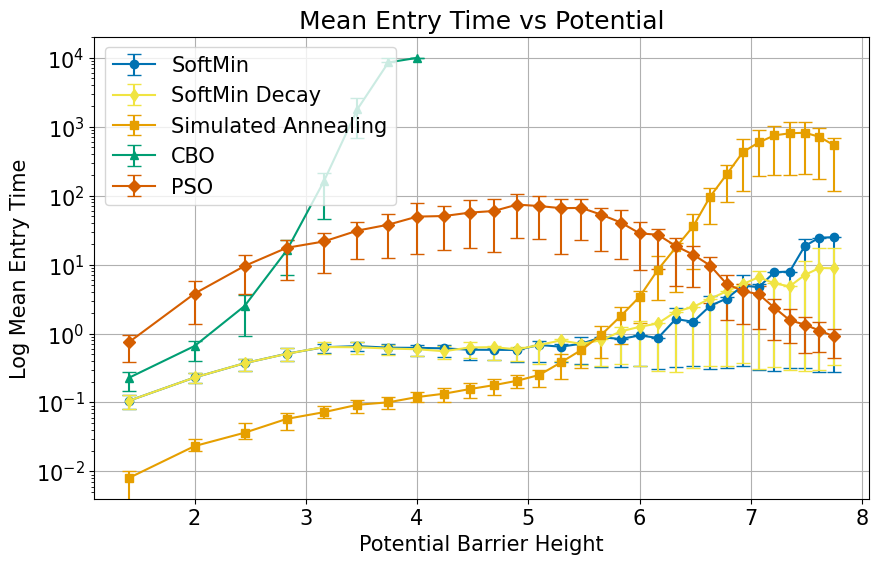
\includegraphics[width=\linewidth]{images/1dim_decay_big.png}
  \end{minipage}\hfill
  \begin{minipage}{0.32\textwidth}
    \centering
    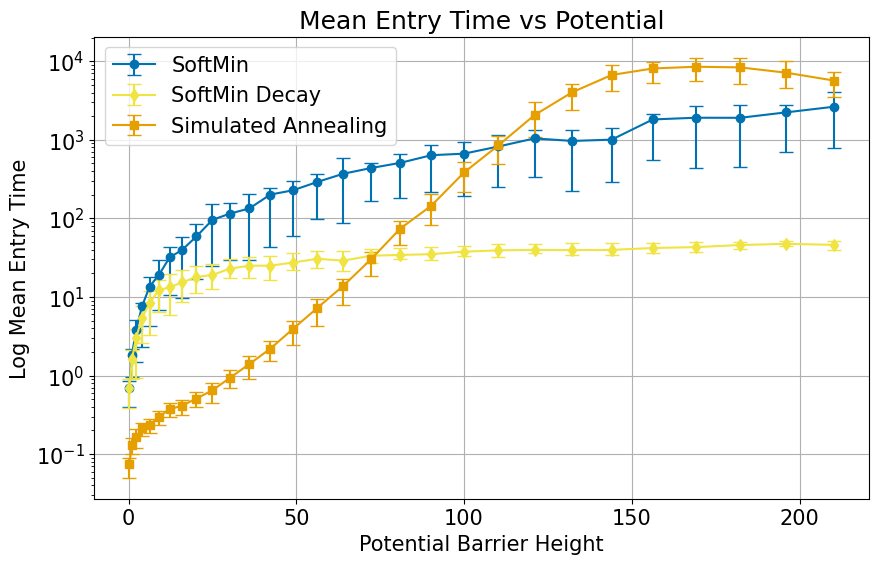
\includegraphics[width=\linewidth]{images/2dim_big.png}
  \end{minipage}\hfill
  \begin{minipage}{0.32\textwidth}
    \centering
    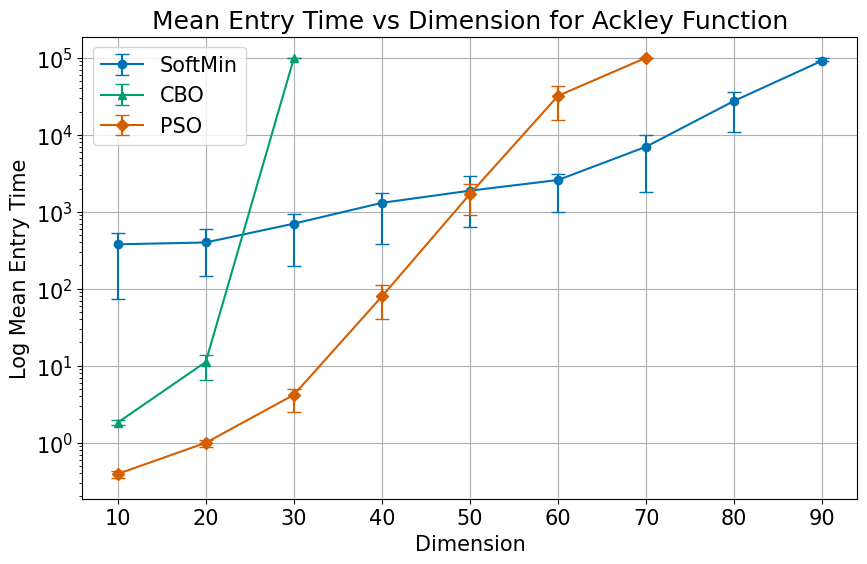
\includegraphics[width=\linewidth]{images/high_dim.png}
  \end{minipage}
  \caption{Legacy diagnostic plots from the submitted version.  These plots must be regenerated under the cost-matched protocol above; the left panel must use an asymmetric double well.}
  \label{fig:experiments}
\end{figure*}

\section{Conclusion}
We introduced a Langevin system on particle space driven by the joint potential \(U_\beta=nJ_\beta\).  The mathematically defensible conclusions are narrower than those in the submitted version.  The interaction produces a sign-changing scalar multiplier of each local gradient; consensus at strict local minima remains stable; noncritical zero-rate equilibria are unstable; the best ensemble value inherits a gradient-flow rate under a Polyak--\L{}ojasiewicz condition; and an explicit frozen-background path yields an \(O(\beta^{-1})\) upper bound on the small-noise basin-exit exponent.  These results do not prove global convergence, exact Eyring--Kramers asymptotics, or permanent optimizing/exploratory roles for designated particles.

\subsection{Limitations and future work}
A complete metastability analysis would need to identify the relevant critical points of \(U_\beta\), establish matching lower and upper bounds for the quasipotential, and analyze the time-inhomogeneous case \(\beta_t\).  The empirical claims also require cost-normalized comparisons, broader benchmark suites, and sensitivity analyses.  Mean-field limits and discretization-error bounds are additional open directions.

\bibliographystyle{plain}  
\bibliography{references}  

\newpage
\appendix
\onecolumn
\section{Technical proofs}
\label{apx:technical-proofs}

\subsection{Differential identities and equilibrium geometry}

\begin{lemma}[Component gradient and special Hessian blocks]
\label{lem:derivative-of-J-proof}
Let \(U_\beta=nJ_\beta\), and define \(a_k\) as in \eqref{eq:softmin-gradient}.  Then
\[
 \nabla_{x_k}U_\beta(\mathbf{x})=a_k(\mathbf{x})\nabla f(x_k).
\]
If \(\mathbf{x}=(z,\ldots,z)\) and \(\nabla f(z)=0\), then all mixed Hessian blocks vanish and
\[
 \nabla^2_{x_kx_k}U_\beta(\mathbf{x})=\nabla^2f(z).
\]
If \(a_k(\mathbf{x})=0\) and \(\nabla f(x_k)\neq0\), then
\[
 \nabla^2_{x_kx_k}U_\beta(\mathbf{x})
 =-n\beta w_k(\mathbf{x})\nabla f(x_k)\nabla f(x_k)^\top.
\]
\end{lemma}

\begin{proof}
Differentiating \(J_\beta=\sum_i w_i f(x_i)\) gives
\[
 \nabla_{x_k}J_\beta
 =w_k\bigl[1-\beta(f(x_k)-J_\beta)\bigr]\nabla f(x_k),
\]
and multiplying by \(n\) yields the first identity.  At consensus, \(w_k=1/n\), \(a_k=1\), and every term containing \(\nabla f(z)\) vanishes, leaving the stated diagonal Hessian.  Finally, differentiate \(\nabla_{x_k}U_\beta=a_k\nabla f(x_k)\).  At \(a_k=0\), the Hessian term \(a_k\nabla^2f(x_k)\) vanishes.  Writing \(q_k=1-\beta(f(x_k)-J_\beta)\), the condition \(a_k=0\) implies \(q_k=0\), and
\[
 \nabla_{x_k}a_k=nw_k\nabla_{x_k}q_k
 =-n\beta w_k\nabla f(x_k),
\]
because \(\nabla_{x_k}J_\beta=(a_k/n)\nabla f(x_k)=0\).  Substitution gives the final formula.
\end{proof}

\begin{proof}[Proof of Theorem \ref{thm:stable-stationary-points}]

Set
\[
    U_\beta(\mathbf x):=nJ_\beta(\mathbf x).
\]
The particle system is the gradient flow
\[
    \dot{\mathbf x}=-\nabla U_\beta(\mathbf x).
\]

We first recall two elementary consequences of local asymptotic stability.

First, \(\bar{\mathbf x}\) must be a local minimum of \(U_\beta\). Indeed, along every trajectory,
\[
    \frac{d}{dt}U_\beta(\mathbf x(t)) = -\|\nabla U_\beta(\mathbf x(t))\|^2 \leq 0.
\]
If points \(\mathbf y\) arbitrarily close to \(\bar{\mathbf x}\) satisfied
\[
    U_\beta(\mathbf y)<U_\beta(\bar{\mathbf x}),
\]
then the trajectory starting from \(\mathbf y\) could not converge to \(\bar{\mathbf x}\), since its energy could never increase to \(U_\beta(\bar{\mathbf x})\). This would contradict local attraction. Second, \(\bar{\mathbf x}\) must be an isolated equilibrium. Otherwise, there would exist distinct equilibria converging to \(\bar{\mathbf x}\); the corresponding constant trajectories would not converge to \(\bar{\mathbf x}\).

\paragraph{Step 1: every particle is at a critical point of \(f\).}

The gradient of \(U_\beta\) with respect to the \(k\)-th particle is
\[
    \nabla_{x_k}U_\beta(\mathbf x) = a_k(\mathbf x)\nabla f(x_k).
\]
Hence, at an equilibrium,
\[
    a_k(\bar{\mathbf x})\nabla f(\bar x_k)=0.
\]

Suppose that, for some \(k\),
\[
    \nabla f(\bar x_k)\neq0.
\]
The equilibrium condition then implies
\[
    a_k(\bar{\mathbf x})=0.
\]
At such a point, the \(k\)-th diagonal block of the Hessian of \(U_\beta\) is
\[
    \nabla^2_{x_kx_k}U_\beta(\bar{\mathbf x}) = -n\beta w_k(\bar{\mathbf x}) \nabla f(\bar x_k)\nabla f(\bar x_k)^\top.
\]
In particular,
\[
    \begin{aligned}
        &\nabla f(\bar x_k)^\top \nabla^2_{x_kx_k}U_\beta(\bar{\mathbf x}) \nabla f(\bar x_k) \\
        &\qquad = -n\beta w_k(\bar{\mathbf x}) \|\nabla f(\bar x_k)\|^4 <0.
    \end{aligned}
\]
Thus \(U_\beta\) decreases along a sufficiently small perturbation of the \(k\)-th particle in the direction \(\nabla f(\bar x_k)\). This contradicts the fact that \(\bar{\mathbf x}\) is a local minimum of \(U_\beta\).

Therefore,
\[
    \nabla f(\bar x_k)=0 \qquad \text{for every }k.
\]

\paragraph{Step 2: the zero-prefactor case is impossible.}

Fix \(k\), freeze the other \(n-1\) particles at their equilibrium positions, and regard \(U_\beta\) as a function of the scalar energy \(r=f(x_k)\). More precisely, define
\[
    \Psi_k(r) := n \frac{r e^{-\beta r} + \sum_{j\neq k} f(\bar x_j)e^{-\beta f(\bar x_j)}}{e^{-\beta r} + \sum_{j\neq k} e^{-\beta f(\bar x_j)}}.
\]
Then
\[
    U_\beta (\bar x_1,\ldots,x_k,\ldots,\bar x_n) = \Psi_k(f(x_k)).
\]
Furthermore,
\[
    \Psi_k'(f(\bar x_k)) = a_k(\bar{\mathbf x}).
\]

Assume that
\[
    a_k(\bar{\mathbf x})=0.
\]
A direct differentiation gives
\[
    \Psi_k''(f(\bar x_k)) = -n\beta w_k(\bar{\mathbf x})<0.
\]
Hence \(r=f(\bar x_k)\) is a strict local maximum of \(\Psi_k\).

There are now two possibilities.

If \(f\) is not locally constant near \(\bar x_k\), then there exist points \(y\) arbitrarily close to \(\bar x_k\) such that
\[
    f(y)\neq f(\bar x_k).
\]
For all sufficiently close such points,
\[
    \Psi_k(f(y)) < \Psi_k(f(\bar x_k)).
\]
Equivalently,
\[
    U_\beta(\bar x_1,\ldots,y,\ldots,\bar x_n) < U_\beta(\bar{\mathbf x}),
\]
contradicting local minimality of \(U_\beta\).

If \(f\) is locally constant near \(\bar x_k\), then
\[
    \nabla f(y)=0
\]
for every \(y\) in a neighborhood of \(\bar x_k\). Replacing \(\bar x_k\) by any such \(y\) leaves all function values, Gibbs weights, and prefactors unchanged. It therefore produces a continuum of equilibria arbitrarily close to \(\bar{\mathbf x}\), contradicting the isolation of an asymptotically stable equilibrium.

Thus
\[
    a_k(\bar{\mathbf x})\neq0 \qquad \text{for every }k.
\]

\paragraph{Step 3: classification according to the prefactor sign.}

Suppose first that
\[
    a_k(\bar{\mathbf x})>0.
\]
Since
\[
    \Psi_k'(f(\bar x_k))>0,
\]
the function \(\Psi_k\) is strictly increasing in a neighborhood of \(f(\bar x_k)\).

If \(\bar x_k\) were not a local minimum of \(f\), there would exist a sequence \(y_m\to\bar x_k\) such that
\[
    f(y_m)<f(\bar x_k).
\]
For sufficiently large \(m\), strict monotonicity would give
\[
    \Psi_k(f(y_m)) < \Psi_k(f(\bar x_k)),
\]
and therefore
\[
    U_\beta(\bar x_1,\ldots,y_m,\ldots,\bar x_n) < U_\beta(\bar{\mathbf x}).
\]
This again contradicts local minimality. Hence \(\bar x_k\) is a local minimum of \(f\).

The case
\[
    a_k(\bar{\mathbf x})<0
\]
is analogous. In this case \(\Psi_k\) is locally decreasing. If \(\bar x_k\) were not a local maximum of \(f\), nearby points with larger objective value would produce smaller values of \(U_\beta\). Thus \(\bar x_k\) must be a local maximum of \(f\).

Since \(n w_k(\bar{\mathbf x})>0\), the sign of \(a_k\) is precisely the sign of
\[
    1-\beta \bigl(f(\bar x_k)-J_\beta(\bar{\mathbf x})\bigr).
\]
Therefore,
\[
    a_k(\bar{\mathbf x})>0 \iff f(\bar x_k) < J_\beta(\bar{\mathbf x})+\frac1\beta,
\]
and
\[
    a_k(\bar{\mathbf x})<0 \iff f(\bar x_k) > J_\beta(\bar{\mathbf x})+\frac1\beta.
\]

\paragraph{Step 4: at least one particle is at a local minimum.}

For every configuration \(\mathbf x\),
\[
\begin{aligned}
    \sum_{k=1}^n a_k(\mathbf x) &= n\sum_{k=1}^n w_k(\mathbf x) \left[ 1-\beta \bigl(f(x_k)-J_\beta(\mathbf x)\bigr) \right] \\
    &= n\left[ 1-\beta \left( \sum_{k=1}^n w_k(\mathbf x)f(x_k) - J_\beta(\mathbf x) \sum_{k=1}^n w_k(\mathbf x) \right) \right] \\
    &=n,
\end{aligned}
\]
because
\[
    \sum_{k=1}^n w_k=1, \qquad \sum_{k=1}^n w_kf(x_k)=J_\beta(\mathbf x).
\]
Thus at least one coefficient \(a_k(\bar{\mathbf x})\) is positive. By the preceding classification, the corresponding particle lies at a local minimum of \(f\).
\end{proof}

\subsection{Proof of the one-dimensional passage theorem}
\label{app:proof-one-dimensional-passage}

\begin{proof}[Proof of Theorem~\ref{thm:transition-time}]
We divide the proof into four steps.

\paragraph{Step 1: geometry of the frozen-background potential.}
Factoring \(e^{-\beta f(z_-)}\) from the Gibbs weights gives
\begin{align*}
    J_\beta(\Gamma(x))
    &=
    \frac{
        e^{-\beta f(x)}f(x)
        +(n-1)e^{-\beta f(z_-)}f(z_-)
    }{
        e^{-\beta f(x)}
        +(n-1)e^{-\beta f(z_-)}
    }
    \\
    &=
    f(z_-)
    +
    \frac{r(x)e^{-\beta r(x)}}{n-1+e^{-\beta r(x)}}.
\end{align*}
Since \(U_\beta=nJ_\beta\), this proves
\[
    U_\beta(\Gamma(x))-U_\beta(\Gamma(z_-))
    =
    u_{n,\beta}(r(x)).
\]

Differentiation yields
\begin{equation}
    u_{n,\beta}'(r)
    =
    \frac{
        ne^{-\beta r}
        \bigl[(n-1)(1-\beta r)+e^{-\beta r}\bigr]
    }{
        (n-1+e^{-\beta r})^2
    }.
    \label{eq:reduced-softmin-derivative}
\end{equation}
Its sign is the sign of
\[
    q(r):=(n-1)(1-\beta r)+e^{-\beta r}.
\]
The function \(q\) is strictly decreasing because
\[
    q'(r)
    =
    -\beta(n-1)-\beta e^{-\beta r}<0.
\]
Moreover,
\[
    q(0)=n>0,
    \qquad
    q(r)\longrightarrow-\infty
    \quad\text{as }r\to\infty.
\]
Therefore \(q\) has a unique zero
\(r_{n,\beta}^{\mathrm c}>0\), and \(u_{n,\beta}\) is increasing before this point and decreasing after it.

For every \(r>0\),
\[
    u_{n,\beta}(r)
    <
    \frac{n}{n-1}r e^{-\beta r}.
\]
Since
\[
    \max_{r\ge0}r e^{-\beta r}
    =
    \frac{1}{e\beta},
\]
we obtain
\[
    B_{n,\beta}
    <
    \frac{n}{e(n-1)\beta}.
\]

\paragraph{Step 2: action required to reach the physical saddle.}
Let
\[
    W_\beta(x):=u_{n,\beta}(r(x)).
\]
A channel path has the form
\(\boldsymbol\phi(t)=\Gamma(\psi(t))\). Since the frozen coordinates remain at the critical point \(z_-\), their drift vanishes along the channel, and the action reduces to
\begin{equation}
    I_{0T}^{\Gamma}(\psi)
    =
    \frac14\int_0^T
    \left|
        \dot\psi(t)+W_\beta'(\psi(t))
    \right|^2dt.
    \label{eq:channel-action}
\end{equation}
The one-dimensional version of \eqref{eq:gradient-action-decomposition} is
\begin{equation}
\begin{aligned}
    I_{0T}^{\Gamma}(\psi)
    &=
    W_\beta(\psi(T))-W_\beta(\psi(0))
    \\
    &\quad+
    \frac14\int_0^T
    \left|
        \dot\psi(t)-W_\beta'(\psi(t))
    \right|^2dt.
\end{aligned}
\label{eq:channel-gradient-action}
\end{equation}

Set
\[
    r_m:=\min\{h,r_{n,\beta}^{\mathrm c}\},
\]
and let \(x_m\in(z_-,s]\) be the unique point satisfying
\(r(x_m)=r_m\). Such a point exists and is unique because \(r\) is strictly increasing on \((z_-,s)\).

Every continuous channel path from \(z_-\) to \(s\) must pass through \(x_m\). Applying \eqref{eq:channel-gradient-action} up to its first hitting time of \(x_m\) gives
\[
    I_{0T}^{\Gamma}(\psi)
    \ge
    W_\beta(x_m)-W_\beta(z_-)
    =
    \widehat B_{n,\beta}(h).
\]

Conversely, this cost is attained in the quasipotential sense by following the reversed gradient flow from \(z_-\) to \(x_m\). If \(x_m<s\), one crosses the critical point \(x_m\) with arbitrarily small additional action and then follows the forward deterministic flow from the right of \(x_m\) toward \(s\). The reversed-gradient part costs exactly
\(W_\beta(x_m)-W_\beta(z_-)\), whereas the forward deterministic part has zero action. Standard finite-time approximations handle the asymptotic approach to the critical points. Hence
\[
    V_{\beta,\mathrm{in}}^\Gamma
    =
    \widehat B_{n,\beta}(h).
\]

Since the full quasipotential is minimized over a larger class of paths,
\[
    V_\beta\bigl(\Gamma(z_-),\Gamma(s)\bigr)
    \le
    \widehat B_{n,\beta}(h).
\]
Finally, for every \(r>0\),
\[
    \frac{u_{n,\beta}(r)}{r}
    =
    \frac{ne^{-\beta r}}{n-1+e^{-\beta r}}
    <1.
\]
If \(h\le r_{n,\beta}^{\mathrm c}\), then
\[
    \widehat B_{n,\beta}(h)=u_{n,\beta}(h)<h.
\]
If \(h>r_{n,\beta}^{\mathrm c}\), then
\[
    \widehat B_{n,\beta}(h)
    =
    u_{n,\beta}(r_{n,\beta}^{\mathrm c})
    <
    r_{n,\beta}^{\mathrm c}
    <
    h.
\]
Thus \(\widehat B_{n,\beta}(h)<h\) in both regimes.

Whenever the hypotheses of the standard Freidlin--Wentzell exit theorem hold for a metastable domain \(D_-\), it gives
\[
    \lim_{\sigma\downarrow0}
    \sigma\log
    \mathbb E_{\bar{\mathbf z}_-}\tau_{D_-}^\sigma
    =
    V_\beta(\bar{\mathbf z}_-,\partial D_-).
\]
If \(\Gamma(x_m)\in\partial D_-\), the preceding channel construction yields the upper bound in \eqref{eq:initial-exit-time-bound}.

\paragraph{Step 3: the Softmin-induced post-saddle well.}
Assume
\[
    h>r_{n,\beta}^{\mathrm c},
    \qquad
    \rho_+<r_{n,\beta}^{\mathrm c}.
\]
At
\[
    \mathbf s:=\Gamma(s),
\]
all particle coordinates are critical points of \(f\). Hence every mixed Hessian block of \(U_\beta\) vanishes.

For the active particle, the channel identity gives
\[
    \partial_{x_1x_1}^2U_\beta(\mathbf s)
    =
    u_{n,\beta}'(h)f''(s).
\]
Since \(h>r_{n,\beta}^{\mathrm c}\), we have
\(u_{n,\beta}'(h)<0\). Since \(s\) is a nondegenerate local maximum of \(f\), we have \(f''(s)<0\). Therefore
\[
    \partial_{x_1x_1}^2U_\beta(\mathbf s)>0.
\]

For a frozen particle \(j\ge2\), the coefficient multiplying
\(f''(z_-)\) in the corresponding diagonal Hessian block is
\[
    a_j(\mathbf s)
    =
    n w_j(\mathbf s)
    \left[
        1-
        \beta\bigl(f(z_-)-J_\beta(\mathbf s)\bigr)
    \right].
\]
Because \(J_\beta(\mathbf s)>f(z_-)\), this coefficient is strictly positive. Since \(f''(z_-)>0\), every frozen-particle block is strictly positive. The Hessian of \(U_\beta\) at \(\mathbf s\) is therefore positive definite, and \(\mathbf s\) is a strict local minimum.

\paragraph{Step 4: passage from the post-saddle well.}
On \((s,z_+)\), the function \(r\) decreases strictly from \(h\) to \(\rho_+\). The assumptions
\[
    \rho_+<r_{n,\beta}^{\mathrm c}<h
\]
therefore imply the existence of a unique
\(\xi_+\in(s,z_+)\) satisfying
\[
    r(\xi_+)=r_{n,\beta}^{\mathrm c}.
\]
Between \(s\) and \(\xi_+\), the reduced potential increases from
\[
    W_\beta(s)=u_{n,\beta}(h)
\]
to
\[
    W_\beta(\xi_+)=B_{n,\beta}.
\]
The same gradient-action argument as in Step 2 gives
\[
    V_{\beta,\mathrm{post}}^\Gamma
    =
    B_{n,\beta}-u_{n,\beta}(h).
\]
Since \(h>r_{n,\beta}^{\mathrm c}\),
\[
    0<u_{n,\beta}(h)<B_{n,\beta},
\]
and hence
\[
    0<
    V_{\beta,\mathrm{post}}^\Gamma
    <
    B_{n,\beta}.
\]
The full quasipotential is again no larger than the action of this channel path, which proves \eqref{eq:post-saddle-quasipotential-bound}.

For \(x\in(\xi_+,z_+)\),
\[
    r(x)<r_{n,\beta}^{\mathrm c},
    \qquad
    u_{n,\beta}'(r(x))>0,
    \qquad
    f'(x)<0.
\]
The active coordinate of the deterministic channel dynamics therefore satisfies
\[
    \dot x
    =
    -u_{n,\beta}'(r(x))f'(x)
    >0.
\]
Since there are no further critical points between \(\xi_+\) and \(z_+\), the active particle is driven toward \(z_+\). This completes the proof.
\end{proof}
\subsection{Best-particle descent}

\begin{proof}[Proof of theorem \ref{thm:rate-of-convergence-minimizing-particle}]
For each \(k\), set
\[
    g_k(t):=f(x_k(t)),
\]
so that
\[
    m(t)=\min_{1\le k\le n}g_k(t).
\]
Let
\[
    I(t):=\{k:g_k(t)=m(t)\}
\]
denote the set of particles attaining the minimum at time \(t\).

We first estimate the effective learning rate of every active minimizer. Fix \(i\in I(t)\). Since
\[
    f(x_i(t))\le f(x_j(t)) \qquad\text{for every }j,
\]
we have
\[
    e^{-\beta_t f(x_j(t))} \le e^{-\beta_t f(x_i(t))}.
\]
Consequently,
\[
    \sum_{j=1}^n e^{-\beta_t f(x_j(t))} \le n e^{-\beta_t f(x_i(t))}
\]
and therefore
\[
    n w_i^{\beta_t}(\mathbf x(t))\ge1.
\]

Moreover, \(J_{\beta_t}(\mathbf x(t))\) is a convex combination of the values \(f(x_j(t))\). Hence
\[
    J_{\beta_t}(\mathbf x(t)) \ge \min_j f(x_j(t)) = f(x_i(t)).
\]
It follows that
\[
    1-\beta_t  \bigl(f(x_i(t))-J_{\beta_t}(\mathbf x(t))\bigr) \ge1.
\]
Combining the two inequalities gives
\[
    a_i(t,\mathbf x(t))\ge1 \qquad\text{for every }i\in I(t).
\]

Along the trajectory of such a particle,
\[
    \begin{aligned}
        \frac{d}{dt}f(x_i(t)) &= \left\langle \nabla f(x_i(t)),\dot x_i(t) \right\rangle \\
        &= -a_i(t,\mathbf x(t)) \|\nabla f(x_i(t))\|^2 \\
        &\le -\|\nabla f(x_i(t))\|^2.
    \end{aligned}
\]

Since each \(g_k\) is continuously differentiable and \(m\) is the minimum of finitely many continuously differentiable functions, \(m\) is locally Lipschitz. In particular, \(m\) is absolutely continuous on every bounded time interval and differentiable for almost every \(t\ge0\).

Fix a time \(t\) at which \(m\) is differentiable, and choose \(i\in I(t)\). Since
\[
    g_i(s)-m(s)\ge0 \qquad\text{for all }s,
\]
and
\[
    g_i(t)-m(t)=0,
\]
the differentiable function \(g_i-m\) has a local minimum at \(t\). Consequently, \( g_i'(t)=m'(t). \)
Therefore, for almost every \(t\ge0\) and every \(i\in I(t)\),
\[
\begin{aligned}
    m'(t) &= \frac{d}{dt}f(x_i(t)) \\ 
    &= -a_i(t,\mathbf x(t)) \|\nabla f(x_i(t))\|^2 \\
    &\le -\|\nabla f(x_i(t))\|^2 \le0,
\end{aligned}
\]
where we used \(a_i(t,\mathbf x(t))\ge1\) for every particle attaining the ensemble minimum.

Since \(m\) is absolutely continuous, for every \(0\le s\le t\),
\[
    m(t)-m(s) = \int_s^t m'(r)\,dr \le0.
\]
Hence \(m\) is nonincreasing. In particular,
\[
    f(x_i(t))=m(t)\le m(0) \qquad \text{for every }i\in I(t),
\]
so every active minimizing particle belongs to the sublevel set
\[
    S_0=\{x\in\mathbb R^d:f(x)\le m(0)\}.
\]

The Polyak--\L{}ojasiewicz inequality therefore gives, for almost every \(t\ge0\) and every \(i\in I(t)\),
\[
    \|\nabla f(x_i(t))\|^2 \ge 2\mu\bigl(f(x_i(t))-f_\star\bigr) = 2\mu\bigl(m(t)-f_\star\bigr).
\]
Thus
\[
    m'(t) \le -2\mu\bigl(m(t)-f_\star\bigr)
\]
for almost every \(t\ge0\).

Define
\[
    y(t):=e^{2\mu t}\bigl(m(t)-f_\star\bigr).
\]
The function \(y\) is absolutely continuous, and for almost every \(t\ge0\),
\[
    y'(t)= e^{2\mu t} \left[ m'(t)+2\mu\bigl(m(t)-f_\star\bigr) \right] \le0.
\]
Hence \(y(t)\le y(0)\), which yields
\[
    m(t)-f_\star \le e^{-2\mu t}\bigl(m(0)-f_\star\bigr), \qquad t\ge0.
\]
\end{proof}

\section{Experimental protocol for the major revision}
\label{app:hyperparameters}

\subsection{Benchmark matrix}
The final revision should report at least the following matrix of problems and dimensions.  Shifted and rotated variants prevent methods from exploiting coordinate alignment.
\begin{table}[H]
\centering
\begin{tabular}{lll}
\toprule
Family & Dimensions & Primary diagnostic \\
\midrule
Tilted double well & 1 & basin exit and role switching \\
Unbalanced multiwell & 2, 5, 10 & controlled barrier crossing \\
Ackley / Rastrigin / Griewank & 10, 30, 50, 100 & multimodal scaling \\
Rosenbrock / L\'evy & 10, 30, 50 & narrow valleys and nonseparability \\
Rotated benchmark suite & 10, 20, 40 & robustness to coordinate rotation \\
\bottomrule
\end{tabular}
\caption{Minimum benchmark coverage required before resubmission.}
\end{table}

\subsection{Cost accounting}
For each run, record objective evaluations \(N_f\), gradient evaluations \(N_g\), wall-clock time, and peak memory.  For Softmin and independent Langevin, one synchronous step with \(n\) particles costs \(n\) objective and \(n\) gradient evaluations unless values are reused.  For gradient-free CBO and standard PSO, report \(N_g=0\) rather than treating an iteration as cost-equivalent to a gradient step.  Present results under fixed \(N_f\) and fixed \(N_g\) budgets, and include evaluations-to-target ECDFs.

\subsection{Tuning and sensitivity}
Use an equal tuning budget for every method.  At minimum, tune or sweep the particle count, step size, noise level, initial inverse temperature, and schedule rate.  Repeat the main table with at least three discretization step sizes.  Report medians and interquartile ranges over independent seeds, together with bootstrap confidence intervals for success probabilities.

\subsection{Mechanism ablation}
Compare the original coefficient \(a_k\) with \((a_k)_+\) and \(|a_k|\).  The first removes exploratory ascent; the second preserves magnitude but forces descent.  Plot the time-dependent proportions of particles in the regimes \(a_k<0\), \(0\le a_k<1\), and \(a_k\ge1\).  Without this ablation, the empirical section does not isolate the proposed mechanism.

\end{document}